% !Mode:: "TeX:UTF-8"

\chapter{基于深度学习的超像素分割和图像分割}

\begin{figure*}[h]
\begin{center}
%\fbox{\rule{0pt}{2in} \rule{.9\linewidth}{0pt}}
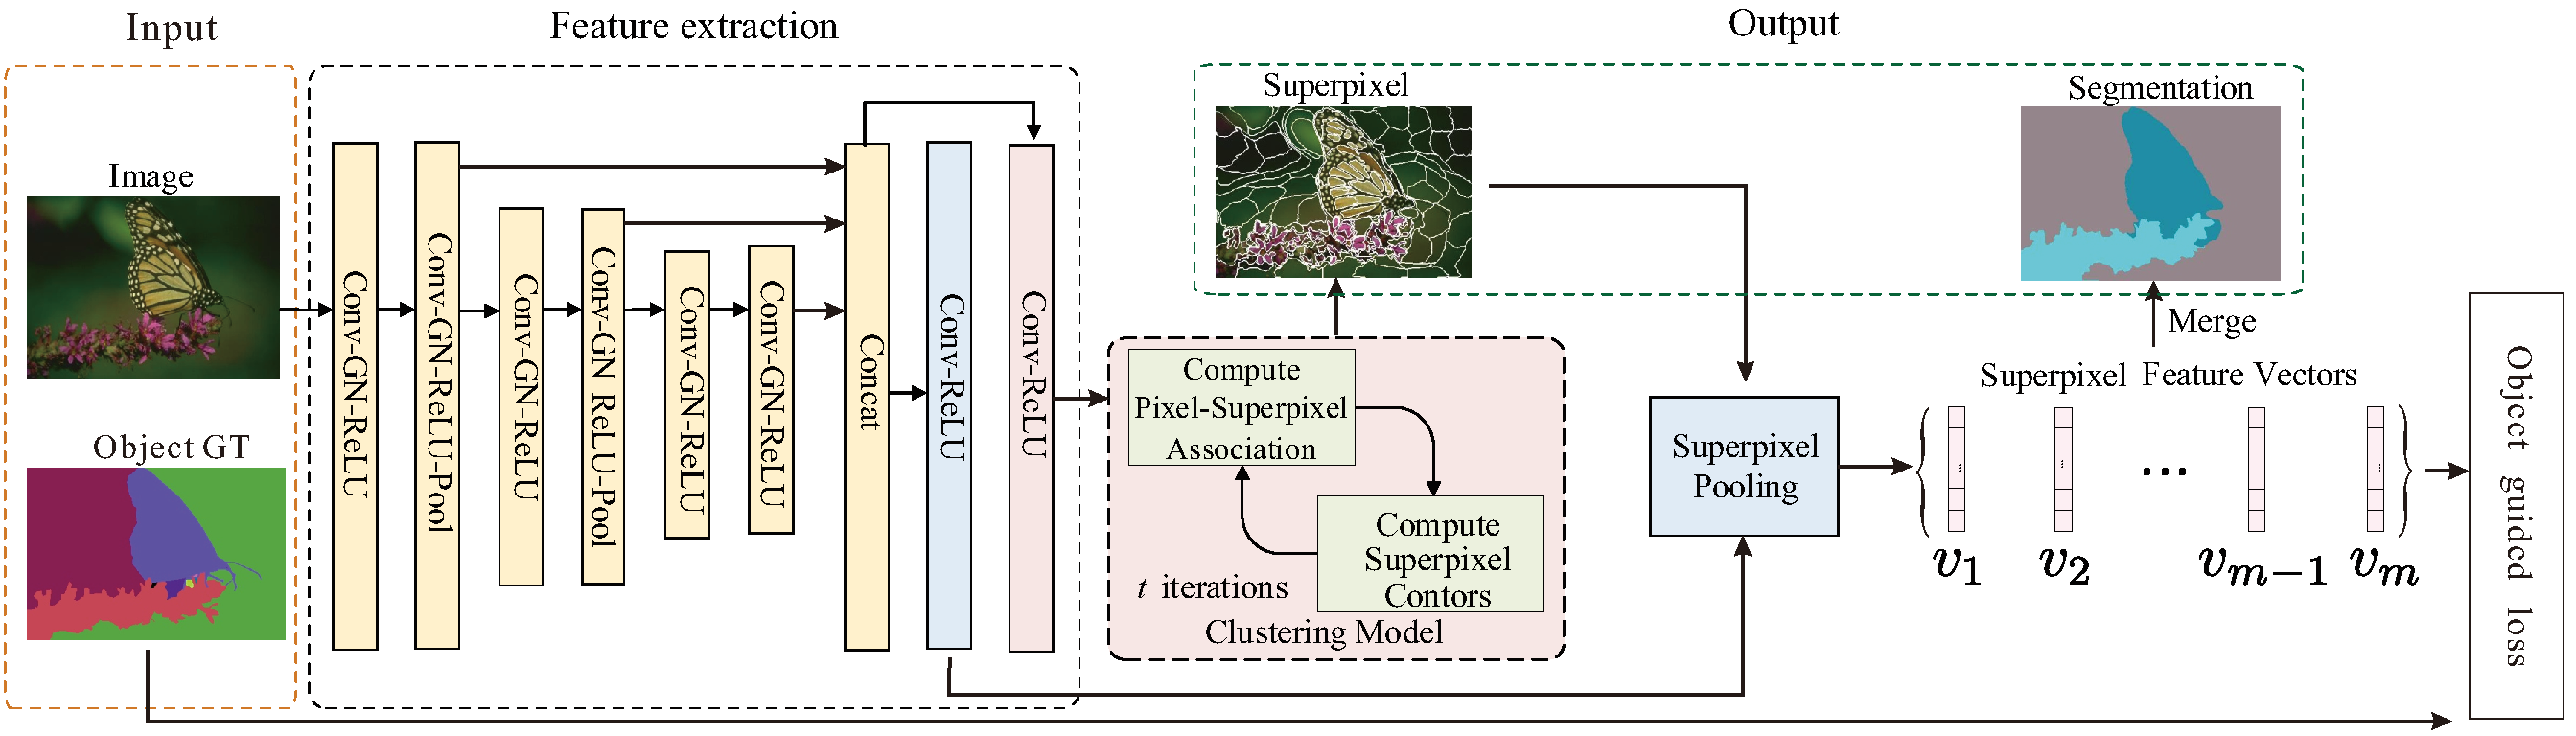
\includegraphics[width=1\textwidth]{figures/img/pipeline.pdf}
\end{center}
\vspace{-5mm}
\caption{算法流程图。对于给定的图像,我们的算法同时生成超像素和图像分割。输入图像首先被输送到一个特征提取网络,该网络由一系列卷积层、归一化(GN)和ReLU操作组成。然后将提取的特征输入可微聚类模块,生成超像素。超像素池用于获取超像素特征向量。最后通过合并相似度高的超像素实现图像分割}
\label{Fig.sub.1}
\end{figure*}

如图3-1所示,我们的方法首先从CNN深度网络中学习图像特征,然后我们使用迭代可微分聚类算法模块来获取超像素。接下来,我们通过超像素池化层计算超像素特征向量,并计算相邻超像素之间的相似性。最后,根据相似度判断相邻的两个超像素是否合并。在本节中,我们将详细介绍我们的方法。

\section{超像素生成}

超像素将相似像素分组为各向同性区域,从而可以提高分割质量和效率。 例如,在DEL算法中,作者使用SLIC作为图像分割的开始。在本文中,与采用现有的超像素算法进行图像分割的方法不同,我们将超像素生成作为图像分割网络的一部分。为此,我们采用SSN中提出的可微聚类算法模块,以取代SLIC算法中的硬像素-超像素关联。

通常,对于$n$像素的图像\(I\in\mathbb{R}^{n\times 5}\),在CIELAB空间的特征为$I_p=[x,y,l,a,b]$ ,我们希望将其划分为$m$ 个小区域,即将图片分成m个超像素。在介绍在描述软关联之前,我们简要介绍SLIC算法中如何计算像素-超像素硬关联$H = \left \{1, 2, \cdots, m \right \}^{n\times 1}$。给定统一采样的超像素中心$C^{0}$作为初始值,SLIC算法在每次迭代$t$中计算每个像素$p$处的新超像素分配,
\begin{equation}\label{eqn:hardassn}
H_{p}^{t} =  \mathop{{{\rm argmin}}}\limits_{{i\in\{ 1, 2, \cdots ,m \} }}\left\|I_{p}-C_{i}^{t-1}\right\|_2,
\end{equation}
其中$\|\cdot\|_2$表示输入向量的$\ell_2$范数,$C_i^{t-1}$表示超像素中心$i$的特征,该特征通过对第$t$次迭代后,计算属于该超像素中心的像素的特征平均值来获取。

由于(3-1)获取像素-超像素硬关联H的操作是不可微的,因此SLIC无法直接集成到神经网络中。 在我们算法中的用到的可微分聚类算法模块,其将硬像素-超像素硬关联H替换为软关联Q。与原始SLIC相似,它在每次迭代中具有以下两个核心步骤:

1.	像素-超像素关联计算。第t次迭代中像素p及其相邻超像素i之间的关联计算如下:
\begin{equation}
Q_{pi}^{t} = e^{-\left \| F_{p}-C_{i}^{t-1}\right \|_2^2},
\end{equation}
其中\(F_{p}\)是像素$p$的深层特征。 在我们的情况下,它来自我们网络的特征提取模块。\(Q_{pi}^{t}\)是$t$次迭代后像素$p$与超像素中心$i$之间的距离。

2.	超像素中心更新。新的超像素聚类中心是根据像素特征的加权总和得出的,
\begin{equation}
C_{i}^{t} = \frac{1}{Z_{i}^{t}}\sum_{p}Q_{pi}^{t}F_{p},
\end{equation}
其中$Z_{i}^{t}$表示归一化过程,即$Z_{i}^{t} = \sum\nolimits_{p}Q_{pi}^{t} $ 。

将这两个步骤迭代数次(在本文中,设定迭代次数为10次),最终得到像素-超像素软关联\(Q\in\mathbb{R}^{n\times m}\)。与(3-1)相似,我们需要计算硬关联映射$H'\in \mathbb{R}^{n\times 1}$,最终得到像素$p$的超像素标签,
\begin{equation}
H'_{p} =  \mathop{{{\rm argmax}}}\limits_{{i \in \left\{ 1, \cdots ,m \right\} }}Q_{pi}.
\label{equation.3}
\end{equation}

值得注意的是,这种硬关联的计算是不可微的。因此在我们的算法中,这一步不参与反向传播。在实验中,我们发现计算像素和超像素聚类中心之间的软关联非常耗时。与SLIC相似,我们只是计算每个像素到周围超像素聚类中心的距离,大大减少了计算时间。

\section{超像素相似度}
在获得超像素之后,我们需要测量它们之间的相似性。超像素的特征可以用超像素池来计算,它实际上是计算属于某个超像素的像素特征的平均值。在我们的算法中,当执行超像素池时,我们使用了不同于在超像素生成中使用的像素特征,如图3-1所示,使用浅蓝色矩形所表示的图像特征。其背后的原因是,超像素不包含语义信息,而图像分割却包含语义信息,因此这两种任务的特征是不同的。我们在实验中通过比较超像素和图像分割的结果以及该算法的一个变体(ours-conv7)来验证这一思想。参考第4.1了解更多细节。

获取超像素后,我们假设超像素的数量为M,将超像素集合表示为$\mathcal{S}=\{S_{1},S_{2},\cdots ,S_{m}\}$,根据图3-1所示,我们所得到的超像素进行超像素池化操作,得到对应超像素的特征向量$\{ v_{1},v_{2},\cdots,v_{m}\}$。超像素池化操作表示如下:
\begin{equation}
v_{i} = \frac{1}{|S_{i}|}\sum_{p\in S_{i} }F'_{p},
\end{equation}
其中,$F'_{p}$ 表示在超像素池中使用的像素$p$的特征向量。

相邻超像素i和超像素j的相似度可以由如下公式获得:
\begin{equation}\label{eqn:sim}
s_{ij} = \frac{2}{1+{\rm exp}\left ( \left \| v_{i}-v_{j}\right \|_{1}\right )},
\end{equation}

其中$s_{ij}$的范围是$[0,1]$。$s_{ij}$值越大,超像素$i$和$j$的相似性越高。当$v_{i}$和$v_{j}$非常相似时,$s_{ij}$接近1,相反,当$v_{i}$和$v_{j}$极为不同时,它接近于0。我们根据相似度$s_{ij}$决定是否合并超像素$i$和$j$。

\section{损失函数}

我们假设同一分割区域内的超像素对之间的相似性大于不同分割区域中的超像素对的相似性。基于(3-6)中定义的相似性度量,我们定义的损失函数如下:
\begin{equation}
\begin{split}
 L =  - \sum_{S_{i}\in S}\sum_{S_{j}\in \mathcal{R}_{i}}   \left[   { \left(
 1  -\alpha  \right)\cdot l_{ij}\cdot \log \left( s_{ij} \right)  } \right. \\
 \left. {  + \alpha \cdot \left( 1-l_{ij}\right) \cdot \log \left( 1- s_{ij}\right)  }   \right],
 \label{equation.6}
\end{split}
\end{equation}
其中$\mathcal{R}_{i}$是超像素$S_{i}$的相邻的超像素集合,$S_i$表示$S_i$和$S_j$是否属于同一个分割区域。在实际应用中,$l_{ij}$ 是由所获得的超像素集和数据集提供的真值来计算的。在$S_i$和$S_i$属于同一分割区域的情况下,$l_{ij} = 1$;否则,$l_{ij} = 0$。

注意,对于不同的输入图像,$l_{ij}$ 的矩阵是不同的。因此,训练阶段的小批量大小必须设置为1,即一次只向网络中输入一张图像。参数$\alpha$表示在真值中属于同一区域的超像素对的比例,用于平衡正样本和负样品。通过将$|Y_+|$ 表示为属于同一区域的超像素对的数目,将$|Y|$表示为超级像素对的总数,通过$\alpha  = \left | Y_{+}\right | / \left | Y \right |$ 来计算。通过反向传播,图像分割也指导了超像素分割。

\section{超像素融合}

通过合并相似的超像素得到最终的图像分割。我们利用相邻超像素之间的相似性和一个预先设定的阈值T来确定两个相邻超像素是否合并。算法1概述了超像素合并的计算步骤。
\begin{algorithm}[h]
  \caption{Superpixel merging algorithm}
  \textbf{Input}: $s$ : similarity;
  \hspace*{2em} $T$ : similarity threshold;\\
  \hspace*{2.5em} $\mathcal{S}=\{S_{1}, S_{2},\cdots, S_{m}\}$ : superpixels.\\
  \textbf{Output}: Segmentation $\mathcal{S}$.
  \begin{algorithmic}[1]
    \For{each $S_{i}\in \mathcal{S}$}
    \State Construct adjacent superpixel set $\mathcal{R}_{i}\subset \mathcal{S}$ of $S_i$;
        \For{each $S_{j}\in R_{i}$}
            \If {$s_{ij} > T$}
                \State$S_{i} \gets S_{i}\cup S_{j}$, $\mathcal{S} \gets \mathcal{S} \setminus S_{j}$ ;
                \State Update $\mathcal{R}_i$ ;
            \EndIf
        \EndFor
    \EndFor
    \label{algorithm1}
  \end{algorithmic}
\end{algorithm}

\section{网络结构}

图3-1显示了我们的网络结构。用于特征提取的CNN网络由卷积层、组规范化(GN)和ReLU激活函数组成。我们将GN中的组数设置为8。在第2层和第4层卷积后,我们使用最大池来增加感受野。对第4层和第6层的输出进行采样,然后与第2层的输出连接,以丰富提取的特征。我们使用3$\times $3卷积滤波器将输出通道设置为每层64个。

注意,考虑到网络中每个小批量的大小必须为1,我们用GN替换了广泛使用的批处理规范化(BN)层。BN操作是深度学习发展中的一个里程碑式的技术,使各种网络能够进行训练。然而,沿着批处理维度进行规范化会带来问题——当批处理大小变小时,BN的错误会迅速增加,这是由于批次统计估计不准确造成的。相反,GN将通道分成组,并计算每组中的均值和方差进行归一化。GN的计算是独立于批量大小的,其精度在较大的批量范围内是稳定的。在实验中,我们还比较了用BN和GN作为归一化的结果。

在多任务学习中,不同层次的任务需要不同的图像特征,如supernet。对于超像素生成和图像分割这两个不同层次的任务,我们进一步对上一步得到的图像特征进行卷积运算,得到不同的特征向量,以满足不同任务的需要。具体来说,对于超像素生成任务,我们使用核大小为3$\times $3的卷积层来获得30个通道的特征向量。对于图像分割任务,我们首先对256个输出通道进行3$\times $3卷积运算,然后使用1$\times $1卷积核得到64个通道的特征向量。如图3-1所示,我们将得到的特征向量分别输入到后续的可微聚类算法模块和超像素池层,然后利用所提出的相应的损失函数对网络进行训练。

\section{实施细节}

我们基于Caffe框架来搭建神经网络,这是一个非常有效的深度学习框架,广泛应用于学术界和工业界。所有代码都是用C++和Python包装编写的。

对于超级像素的生成,就像在原始的SLIC算法中一样,我们在(3-4)之后的每个超级像素簇内的像素之间加强空间连通性。通过将小于某个阈值的超像素与周围的超级像素合并,然后为每个空间连接的组件分配一个唯一的聚类ID来实现的。对于图像分割,我们在合并后进行空间连通性增强操作。需要注意的是,加强空间连通性的运算是不可微的,我们只把它当作后处理,而不加入神经网络。

我们使用BSDS500数据集作为我们的训练和测试数据,该数据集已在图像分割领域得到广泛应用。由于BSDS500中训练样本数量较少,训练时需要进行数据扩充。我们将每一个真值作为一个单独的样本,即对于每一对图像和真值,我们将其作为训练样本提供给网络。通过这种方式,我们得到了1633对训练/验证对和1063对测试对。另外,我们采用了两种常用的数据扩充策略,即翻转和裁剪。具体地说,在训练阶段,我们将图像左右翻转,随机地将图像裁剪成201$\times $201大小的图像块,进行数据增强。采用Adam优化我们的网络。基本学习率设置为1e-5,生成的超级像素数设置为100。动量设置为0.99,以在相对较小规模的数据上实现稳定优化,如FCN 中所建议的那样。如第3.5,每个小批量的大小设置为1。

我们进行500K次迭代来训练深度学习模型,并根据验证的准确性选择最终的训练模型。

